%!TeX spellcheck = en-ZA

\documentclass[11pt]{article}

\usepackage[utf8]{inputenc}
\usepackage[margin=1in]{geometry}
\usepackage[english]{babel}
\usepackage{tocloft}
\usepackage{amsmath}
\usepackage{amsfonts}
\usepackage{amssymb}
\usepackage[none]{hyphenat}
\usepackage{graphicx}
\usepackage{fancyhdr}
\usepackage{pdfpages}
\usepackage[font={small,it}]{caption}

\parindent 0ex
\linespread{1.5}
\setlength{\headheight}{30pt}
\setcounter{tocdepth}{1}
\pagestyle{fancy}

\fancyhead{}
%\fancyfoot{}
\fancyhead[L]{\slshape \MakeUppercase{Cryptogen User Manual}}
\rhead{
\includegraphics[width=1cm, height=1cm]{cryogen.png}
\includegraphics[width=1cm, height=1cm]{icon.png}}

\begin{document}
	%insert pdf cover page
	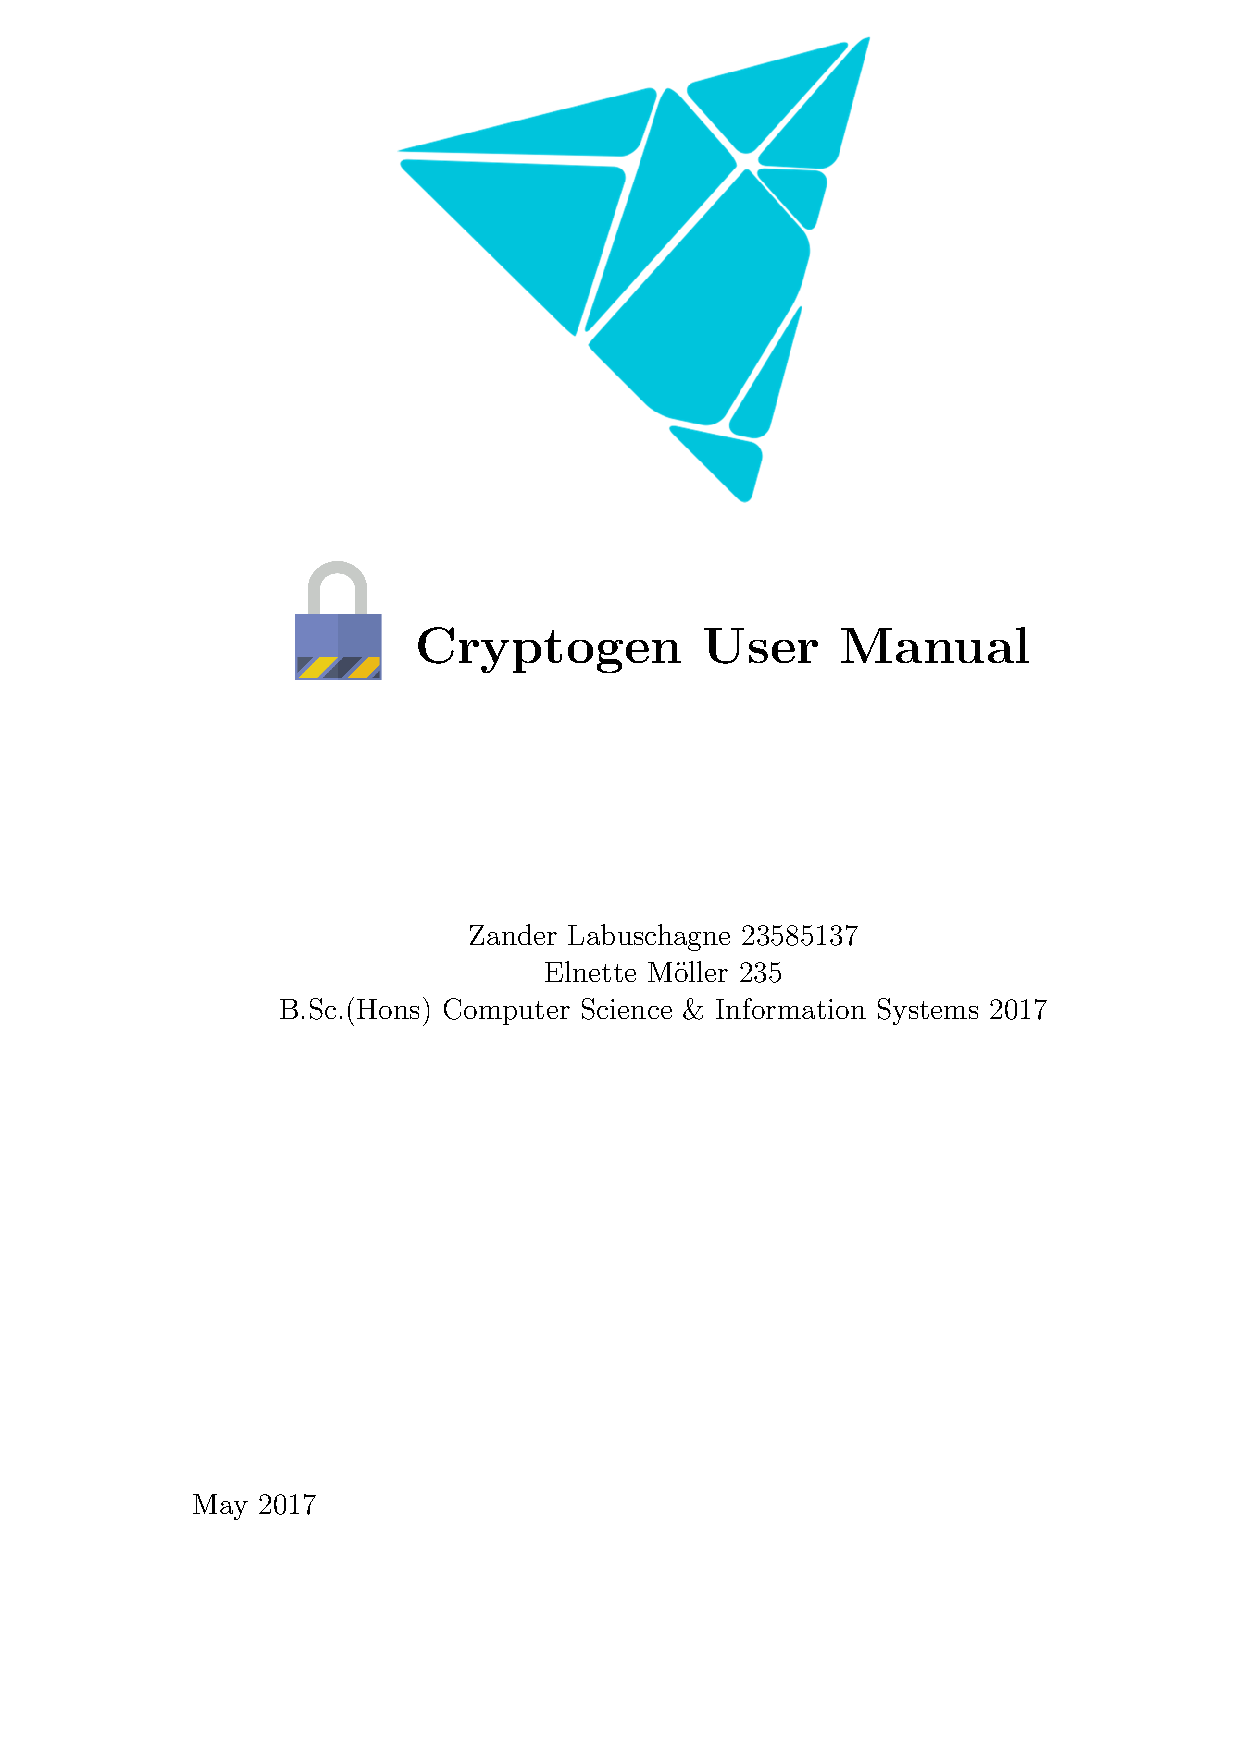
\includepdf[pages={-},offset=0mm 0mm, width=21.5cm, height=28cm]{Cover.pdf}

    \renewcommand{\cftsecleader}{\cftdotfill{\cftdotsep}} % TOC Dotted Lines
    \tableofcontents
    \thispagestyle{empty}
    \clearpage

	%\printglossary[title=Abbreviation]

    \setcounter{page}{1}

	\section{Introduction}
	\subsection{Intended Readership}
	This documented is intended for the users of the Cryptogen application used for the encryption and decryption of messages and files which is developed by two computer science students at the Nort-West University, Zander Labuschagne \& Elnette M\"{o}ller.

	\subsection{Applicability}
	This user manual only applies to version 1.x of the Cryptogen application developed by Zander Labuschagne \& Elnette M\"{o}ller.

	\subsection{Purpose}
	The purpose of this document is to aid the users of the Cryptogen application so they can use it properly and as intended by the developers. This document hopes to clarify any misunderstandings its users might have.

	\subsection{Motivation \& Background}
	Cryptogen is developed as part of the Computer Security module for B.Sc. Computer Science \& Information Systems Honnors students at the North-West University, Potchefstroom Campus. The goal of this project was to provide students with experience in elementary cryptosystems by developing a small
	system which implements different encryption algorithms. It was expected of one to two student to work together and develop an application which satisfies the following requirements:
	\begin{itemize}
		\item Handle encryption and decryption of messages and files.
		\item Graphical interface to simplify the functioning.
		\item Any programming language(s) may be used.
		\item The following algorithms had to be implemented:
		\begin{itemize}
			\item Vigen\`{e}re Cipher
			\item Vernam Cipher
			\item Columnar Transposition Cipher
			\item Own implementation
		\end{itemize}
	\end{itemize}

	\section{User Guide}
	\subsection{Support}
	\subsubsection{Linux}
	This project was partly developed on a GNU/Linux system, more specifically Manjaro ArchLinux 17.01 KDE x86\_64 running Manjaro kernel version 4.11. Linux systems are fully supported and Cryptogen is expected to run flawless on these systems, but is not guaranteed. Any bugs and inconsistencies may be reported to the developers, at least one of the developers aims to maintain this project for UNIX-like systems. A shell script named install.sh is provided which one can run to install the application on a Linux system. The installation adds an application entry to the applications menu or better known as a desktop entry for the application. Since a Java .jar file is provided one can run the .jar executable on Linux systems if Java Runtime Environment 1.8 or higher is installed, \textbf{very important: OpenJDK will not suffice!} but it is more convenient to do the installation and to use the application as intended. One can run the install with the terminal command ``sudo sh install.sh'', if a permission error is encountered first enter the following command before installation: ``sudo chmod +x install.sh'', this will add executable permission to the install script. To be able to read this document a PDF reader is required such as Okular.

	\subsubsection{Windows}
	This project was partly developed on a Windows platform, thus some Windows support is provided such as a GUI specifically adapted for Windows. Many problems or inconsistencies were experienced by the developers when the application was used on a Windows platform such as malfunctioning drag \'n drop, so there is no guarantee that the application will function proporly on Windows systems. It is very complicated to create an installer or portable .exe for Windows from a .jar executable and the little third party software that exists to make this process simpler is very expensive hence no Windows executable or intsaller. There is no guaratee that the developers will address any bugs or problems experienced on Windows systems but feedback is welcome just to keep record of what functions well. Since a Java .jar file is provided one can run the .jar executable on Windows systems if Java Runtime Environment 1.8 or higher is installed. To be able to read this document a PDF reader is required such as Adobe Reader.

	\subsubsection{macOS}
	This application was not yet tested on a macOS system and since the lack of a macOS system from the developers no dedicated installer or macOS executable(.app or .dmg) was made. However at least one of the two developers aims add support for macOS systems in the future. Since a Java .jar file is provided one can run the .jar executable on a macOS system if Java Runtime Environment 1.8 or higher is installed. To be able to read this document a PDF reader is required such as Skim.

	\subsection{Features Overview}
	\subsubsection{Cryptosystems}
	This application currently provides Vigen\`ere, Vernam, columnar transposition ciphers and our own implementation called the Elephant Cipher. Support for more cryptosystems in the future is planned. One can select a cryptosystem to use by choosing one of the options on the top left area, the dot represents the selected cryptosystem.\\

	The Vigen\`ere cipher only encrypts and decrypts english alphabetical characters, and leaves all special characters in their original form since the Vigen\`ere cipher was designed for text or message encryption only. The key used for Vigen\`ere enryption and decryption may only consist of alphabetical characters as seen in \textit{figures \ref{fig:vigenere_message_cipher}} and \textit{\ref{fig:vigenere_message_plain}}, violating this would produce an error.\\

	The Vernam cipher accepts a key containing any characters unlike the Vigen\`ere cipher, this means that the cipher text will also conatin any other characters as well. The Vernam cipher encrypts and decrypts all characters.\\

	The columnar transposition cipher can take a key containg any characters as well and encrypts and decrypts all charcters just like the Vernam cipher does.

	The Elephant cipher is a self implemented cipher designed by the developers of this application, Zander Labuschagne \& Elnette M\"oller. This cipher can not be considered as a sound cryptosystem because it is based on simple cryptosystems of which one is considerd to be unsound in modern days.

	\subsubsection{Message Encryption \& Decryption}
	Encryption and decryption of messages can be done by using the text area. The user may choose a cryptosystem in the box on the top left corner followed by entering a plain text message into the text area and encrypt it with any of the provided encryption algorithms, see \textit{figure  \ref{fig:vigenere_message_cipher}} for an example of encryption of a message by the Vigen\`ere cipher, this results in an encrypted message provided in the same text area after the ``Encrypt Message'' button has been clicked. The user may also enter an encrypted message in the text area and click on the ``Decrypt Message'' button to decrypt the encrypted message, the result which is the decrypted message will be displayed in the same text area. See \textit{figure \ref{fig:vigenere_message_plain}} for an example of message decryption by using the Vigen\`re cipher.\\

\begin{figure}[!htb]
\centering
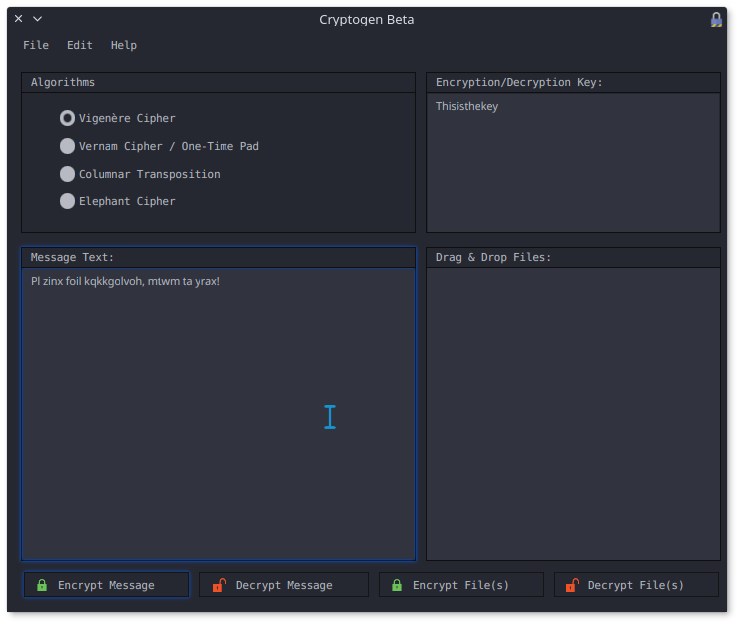
\includegraphics[scale=0.55]{vigenere_message_cipher}
\caption{Vigen\`ere message encryption} % Figuur Naam
\label{fig:vigenere_message_cipher} % label om na figuur te verwys
\end{figure}

\begin{figure}[!htb]
\centering
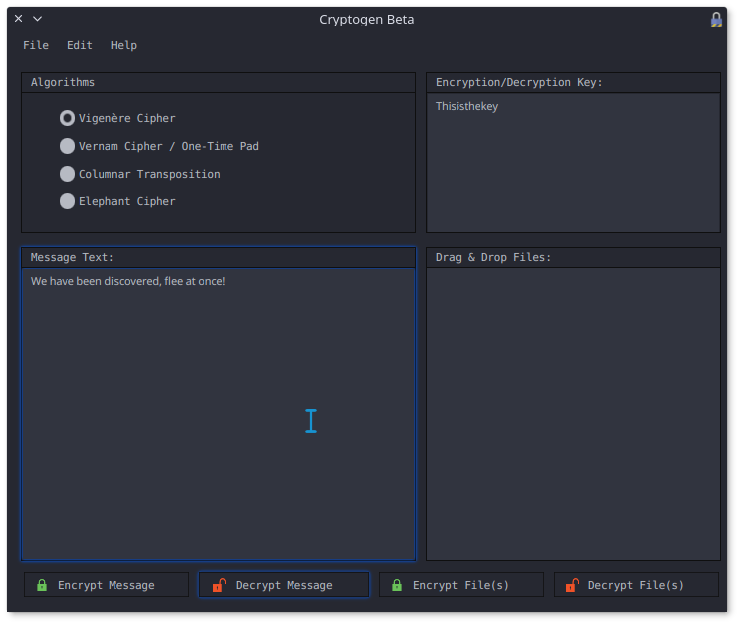
\includegraphics[scale=0.55]{vigenere_message_plain}
\caption{Vigen\`ere message decryption} % Figuur Naam
\label{fig:vigenere_message_plain} % label om na figuur te verwys
\end{figure}


\newpage
	\subsubsection{File(s) Encryption \& Decryption}
	All sorts of video, image, audio and document files may also be encrypted and decrypted(.jpeg, .pdf, .png, .mp4, .flv, .mp4, .docx, .xlsx  etc), there are two ways of doing such, the first is to drag and drop the file(s) into the area on the lower right, as seen in \textit{figure \ref{fig:dragndrop}}, once they are dropped they are ready to be encrypted or decrypted as seen in \textit{figure \ref{fig:files}}. The other way is to select some files or file in your favorite file explorer, on Windows it's Windows Explorer, macOS it's Finder and Linux with KDE it can be Dolphin, and to right click and click on copy or just CTRL+C followed by clicking the File button on the menu inside Cryptogen and choosing ``Paste Files''. After some files are attached, a cryptosystem of choice is chosen and a key is entered in the Key text area on the upper right as in \textit{figure \ref{fig:files}}, they may be encrypted or decrypted by clicking on the ``Encrypt File(s)'' button or the ``Decrypt File(s)'' button respectively. While files are being encrypted or decrypted a progress bar for each file will be displayed, one can move them to different places in the screen to see all progress simulataneously. The size limit of the files depends on the amount of RAM available.\\

	 One can attach one file, multiple files or even multiple folders containing files and more folders, this will encrypt/decrypt all the files inside all the directories, so be careful. When files are encrypted they get the extension ``.cg'' to differentiate them from the normal or decrypted files, the original files are also deleted in the process. When files are decrypted only the encrypted files with the extension ``.cg'' will be selected for decryption, all encrypted files are deleted while the original files are recreated from their encrypted counterparts. Becareful with the total file size, Cryptogen currently puts all files in RAM, so large files may fill up your RAM and may not get encrypted or decrypted, an alternative solution is planned for a future release. To remove attached files one can click on ``File'' followed by clicking on ``Clear Files''.

	 \vspace{4cm}
	\begin{figure}[!htb]
	\centering
	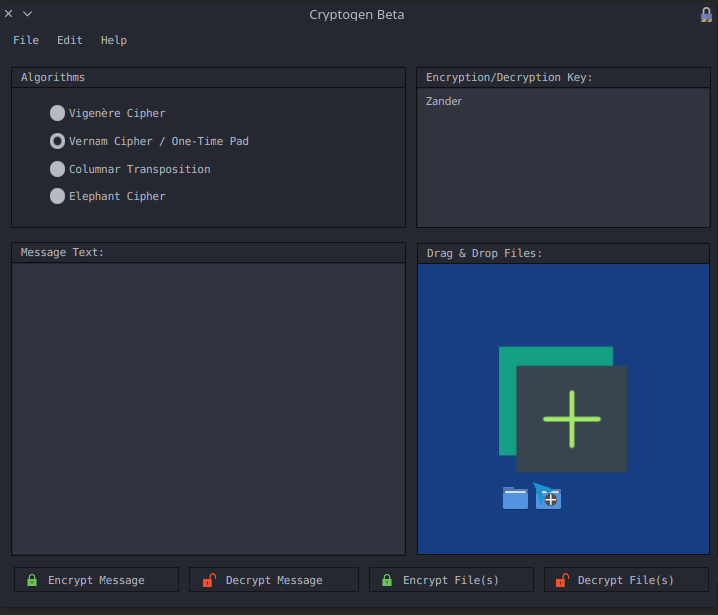
\includegraphics[scale=0.55]{dragndrop.png}
	\caption{Files being dragged into drop area} % Figuur Naam
	\label{fig:dragndrop} % label om na figuur te verwys
	\end{figure}

	\begin{figure}[!htb]
	\centering
	
\includegraphics[scale=0.55]{files.png}
	\caption{Files attached for encryption or decryption} % Figuur Naam
	\label{fig:files} % label om na figuur te verwys
	\end{figure}

\newpage
	\subsubsection{Additional Features}
	The ``Help'' menu provides a button to open this document for help as well as an ``About'' form which displays information about the application as well as the developers. The ``Look and Feel'' menu provides additional look and feels or themes as some might call them, some people have different tastes than others which is why a light look and feel called ``Midna'' is included and two dark look and feels called ``Midna Dark'' and ``Breath''.

	\subsubsection{Technical Features}
	The main programming langauage used is Java with Oracle Java Development Kit version 1.8. A JavaFX framework is used to display the graphical user interface, it includes .fxml files containing the graphical user interface layout, .css files containing information on how the graphical user interface looks and .java files containing code to execute instructions in order to provide functionality into the application. A feature not seen directly is multithreading, when encrypting or decrypting files, each file is encryptes or decrypted on its own thread meaning multiple files can be encrypted or decrypted simultaneously, one can see a progress bar for each file or thread, Appendix B is an example of multithreading. Some might not call this a feature but open source gives many advantages over closed source, this project is open source and available on GitHub, any feedback, criticism or pull requests are welcome.

	\section{Acknowledgements}
	This project was developed and is being maintained with JetBrains IntelliJ IDEA Ultimate edition with a JetBrains student license. This documentation was compiled with \LaTeX. The icons on the ``Encrypt'' and ``Decrypt'' buttons are made by Maxim Basinski from http://www.flaticon.com at http://www.flaticon.com/authors/maxim-basinski and is licensed by Creative Commons BY 3.0 at http://creativecommons.org/licenses/by/3.0/. All other icons are made by Madebyoliver from http://www.flaticon.com at http://www.flaticon.com/authors/madebyoliver and is licensed by Creative Commons BY 3.0. at http://creativecommons.org/licenses/by/3.0/. The default look and feel of Cryptogen is designed after the MidnaDark look and feel for KDE's Plasma theme which is the dark theme used and designed by KaOS, a very beautiful KDE Linux distribution. E-Mail of author, Anke Boersma: demm@kaosx.us KaOS Website: https://kaosx.us. The Midna look and feel is also designed by KaOS and is the default look and feel for KaOS. The Breath look and feel is also a look and feel for KDE's Plasma theme designed by Manjaro, a Linux distribution based on Arch Linux which is very lightweight and embraces simplicity. GitHub is used to do version control over this project since it is easily integratable with JetBrains IntelliJ.

	\section{License}
	Copyright \textcopyright \space 2017 Zander Labuschagne, Elnette M\"oller. Cryptogen is free software: it may redistributed it and/or modified under the terms of the GNU General Public License version 3 as published by the Free Software Foundation. The full license can be viewed in the ``LICENSE'' file.

    \section{Reflection}
		This section contains personal experiences and views from the developer's point of view while the project commenced.\\
		\subsection{Developer \#1: Zander Labuschagne}
		...\\

		\subsection{Developer \#2: Elnette M\"oller}

    \section*{Appendix A: Vigen\`ere Message Decryption Algorithm}
    \addcontentsline{toc}{section}{{}Appendix A: Vigen\`ere Decryption Algorithm}
  	\begin{verbatim}
		/**
		 * Decryption method to decrypt Vigenère encrypted files
		 * @param cipherFile encrypted file to decrypt
		 * @param key key used to decrypt the file
		 * @return the decrypted original file
		 */
		public static void decrypt(File cipherFile, char[] key)
		{
				try
				{
						Path path = Paths.get(cipherFile.getAbsolutePath());
						final byte[] cipherData = Files.readAllBytes(path);
						byte[] plainData = new byte[cipherData.length];

						Progress progress = new Progress("Decryption");
						// In real life this task would do something useful and return
						// some meaningful result:
						Task<byte[]> task = new Task<byte[]>()
						{
								@Override
								public byte[] call() throws InterruptedException
								{
										for(int iv = 0; iv < cipherData.length; iv++)
										{
												updateProgress(iv, cipherData.length);
												plainData[iv] = (byte) ((int) cipherData[iv] - (int) key[iv % key.length]);
										}

										return plainData;
								}
						};
						// binds progress of progress bars to progress of task:
						progress.activateProgressBar(task);

						// in real life this method would get the result of the task
						// and update the UI based on its value:
						task.setOnSucceeded(event ->
						{
								try
								{
										progress.getDialogStage().close();
										FileOutputStream fos = new FileOutputStream(cipherFile.getAbsolutePath().substring(0, cipherFile.getAbsolutePath().length() - 3));
										fos.write(task.getValue());
										fos.close();
										cipherFile.delete();
								}
								catch (FileNotFoundException ex)
								{
										ex.printStackTrace();
										Cryptography.handleException(ex);
								}
								catch(IOException ex)
								{
										ex.printStackTrace();
										Cryptography.handleException(ex);
								}
								catch (Exception ex)
								{
										ex.printStackTrace();
										Cryptography.handleException(ex);
								}
						});

						progress.getDialogStage().show();

						Thread thread = new Thread(task);
						thread.setDaemon(true);
						thread.start();
				}
				catch (IOException ex)
				{
						ex.printStackTrace();
						Cryptography.handleException(ex);
				}
				catch (Exception ex)
				{
						ex.printStackTrace();
						Cryptography.handleException(ex);
				}
		}
  	\end{verbatim}

		\section*{Appendix B: Vernam File Encryption Algorithm}
    \addcontentsline{toc}{section}{{}Appendix B: Vernam File Encryption Algorithm}
\begin{verbatim}
/**
 * Encryption method used to encrypt files with the Vernam cipher
 * @param plainFile file about to be encrypted
 * @param key used to encrypt the file
 * @return the encrypted file
 */
public static void encrypt(File plainFile, char[] key)
{
		try
		{
				Path path = Paths.get(plainFile.getAbsolutePath());
				final byte[] plainData = Files.readAllBytes(path);
				byte[] cipherData = new byte[plainData.length];

				Progress progress = new Progress("Encryption");
				// In real life this task would do something useful and return
				// some meaningful result:
				Task<byte[]> task = new Task<byte[]>()
				{
						@Override
						public byte[] call() throws InterruptedException
						{
								for (int vi = 0; vi < plainData.length; vi++)
								{
										updateProgress(vi, plainData.length);
										cipherData[vi] = (byte) ((int) plainData[vi] ^ (int) key[vi % key.length]);
								}

								return cipherData;
						}
				};
				// binds progress of progress bars to progress of task:
				progress.activateProgressBar(task);

				// in real life this method would get the result of the task
				// and update the UI based on its value:
				task.setOnSucceeded(event ->
				{
						try
						{
								progress.getDialogStage().close();
								FileOutputStream fos = new FileOutputStream(plainFile.getAbsoluteFile() + ".cg");
								fos.write(task.getValue());
								fos.close();
								plainFile.delete();
						}
						catch (FileNotFoundException ex)
						{
								ex.printStackTrace();
								Cryptography.handleException(ex);
						}
						catch (IOException ex)
						{
								ex.printStackTrace();
								Cryptography.handleException(ex);
						}
						catch (Exception ex)
						{
								ex.printStackTrace();
								Cryptography.handleException(ex);
						}
				});

				progress.getDialogStage().show();

				Thread thread = new Thread(task);
				thread.setDaemon(true);
				thread.start();
		}
		catch (IOException ex)
		{
				ex.printStackTrace();
				Cryptography.handleException(ex);
		}
		catch (Exception ex)
		{
				ex.printStackTrace();
				Cryptography.handleException(ex);
		}
}
	\end{verbatim}

		\section*{Appendix C: Encryption of Multiple Directories}
    \addcontentsline{toc}{section}{{}Appendix C: Encryption of Multiple Directories}
    \begin{verbatim}
		/**
     * Handle encryption of multiple files and directories
     * @param files List of files to be encrypted
     */
    private void encryptFiles(List<File> files)
    {
        try
        {
            char[] key = txtKey.getText().toCharArray();
            for (int ii = 0; ii < files.size(); ii++)//Encrypt Each File
            {
                if (files.get(ii).isDirectory())
                    encryptFiles(Arrays.asList(files.get(ii).listFiles()));
                else if (files.get(ii).isFile())
                {
                    if (radVigenere.isSelected())
                    {
                        Cryptography.VigenereCipher.encrypt(files.get(ii), key);
                        method = "Vigenère cipher.";
                    }
                    else if (radVernam.isSelected())
                    {
                        Cryptography.VernamCipher.encrypt(files.get(ii), key);
                        method = "Vernam cipher.";
                    }
                    else if (radColumnarTrans.isSelected())
                    {
                        Cryptography.ColumnarTranspositionCipher.encrypt(files.get(ii), key);
                        method = "columnar transposition.";
                    }
                    else if (radElephant.isSelected())
                    {
                        Cryptography.ElephantCipher.encrypt(files.get(ii), key);
                        method = "Elephant Encryption.";
                    }
                }
            }
        }
        catch (Exception ex)
        {
            ex.printStackTrace();
            handleException(ex);
        }
    }
		\end{verbatim}

		\section*{Appendix D: Drag and Drop Feature}
    \addcontentsline{toc}{section}{{}Appendix D: Drag and Drop Feature}
    \begin{verbatim}
		/**
     * Event necessary to execute before DragDropped may be executed
     * Allows DragDropped to receive files by Copy or Move
     * @param event
     */
    @FXML
    protected void onDragOver(DragEvent event)
    {
        //data is dragged over the target
        if(event.getGestureSource() != stackPane && event.getDragboard().hasString())
            event.acceptTransferModes(TransferMode.COPY_OR_MOVE);
        event.consume();
    }

    /**
     * Method to execute when file is dragged over area
     * @param event
     * @throws IOException
     */
    @FXML
    protected void onDragEntered(DragEvent event)
    {
        pneFilePane.getStyleClass().remove("pneDefault");
        pneFilePane.getStyleClass().remove("pneFilePaneError");
        pneFilePane.getStyleClass().add("pneFilePaneDrag");
    }

    /**
     * Method to execute when file is no longer above area
     * @param event
     */
    @FXML
    protected void onDragExited(DragEvent event)
    {
        pneFilePane.getStyleClass().remove("pneFilePaneDrag");
        pneFilePane.getStyleClass().add("pneDefault");
    }

    /**
     * Method to execute when file(s) is/are dropped in area
     * @param event
     * @throws IOException
     */
    @FXML
    protected void onDragDropped(final DragEvent event) throws IOException
    {
        final Dragboard db = event.getDragboard();
        boolean success = false;
        if (db.hasFiles())
        {
            success = true;
            // Only get the first file from the list
            files = db.getFiles();
            Platform.runLater(new Runnable()
            {
                @Override
                public void run()
                {
                    try
                    {
                        /*for(int i = 0; i < files.size(); i++)
                            System.out.println(files.get(i).getAbsolutePath());*/

                        if(!stackPane.getChildren().isEmpty())
                        {
                            stackPane.getChildren().remove(0);
                        }
                        pneFilePane.getStyleClass().remove("pneFilePaneDrag");
                        pneFilePane.getStyleClass().remove("pneDefault");
                        pneFilePane.getStyleClass().add("pneFilePaneDropped");
                    }
                    catch (Exception ex)
                    {
                        System.out.println(ex.toString());
                    }
                }
            });
        }
        event.setDropCompleted(success);
        event.consume();
    }
		\end{verbatim}

\end{document}
